% !TEX TS-program = pdflatexmk
\documentclass[12pt]{amsart}
\usepackage{multicol}
\usepackage{float}

%\usepackage[parfill]{parskip}    % Activate to begin paragraphs with an empty line rather than an indent

\usepackage[margin=1in]{geometry}


\usepackage{amsmath,amssymb,amsthm,latexsym,graphicx}
\usepackage[normalem]{ulem}
\usepackage{setspace} %used for doublespacing, etc.
\usepackage{hyperref}
\usepackage{cancel}
\usepackage[dvipsnames,usenames]{color}
\usepackage[all]{xy}
\usepackage{fancyhdr}
\pagestyle{fancy}
	\renewcommand{\headrulewidth}{0.5pt} % and the line
	\headsep=1cm
	
\DeclareGraphicsRule{.tif}{png}{.png}{`convert #1 `dirname #1`/`basename #1 .tif`.png}

%Some useful environments.
\newtheorem{theorem}{Theorem}
\newtheorem{corollary}[theorem]{Corollary}
\newtheorem{conjecture}[theorem]{Conjecture}
\newtheorem{lemma}[theorem]{Lemma}
\newtheorem{proposition}[theorem]{Proposition}
\newtheorem{definition}[theorem]{Definition}
\newtheorem{example}[theorem]{Example}
\newtheorem{axiom}{Axiom}
\theoremstyle{remark}
\newtheorem{remark}{Remark}
\newtheorem*{exercise}{Exercise}%[section]

%Some useful shortcuts for our favorite fields
\def\RR{\ensuremath{\mathbb R}} %Note, you can use these WITHOUT entering math mode
\def\NN{\ensuremath{\mathbb N}}
\def\ZZ{\ensuremath{\mathbb Z}}
\def\QQ{{\ensuremath\mathbb Q}}
\def\CC{\ensuremath{\mathbb C}}
\def\EE{{\ensuremath\mathbb E}}

%Some useful shortcuts for formatting lists
\newcommand{\bc}{\begin{center}}
\newcommand{\ec}{\end{center}}
\newcommand{\be}{\begin{enumerate}}
\newcommand{\ee}{\end{enumerate}}
\newcommand{\bi}{\begin{itemize}}
\newcommand{\ei}{\end{itemize}}

%Some useful shortcuts for formatting mathematical symbols
\newcommand{\ol}[1]{\overline{#1}}
\newcommand{\oimp}[1]{\overset{#1}{\iff}} %labeled iff symbol
\newcommand{\bv}[1]{\ensuremath{ \vec{\mathbf{#1}}} } %makes a vector.
\newcommand{\mc}[1]{\ensuremath{\mathcal{#1}}} %put something in caligraphic font
\newcommand{\mpg}[1]{\marginpar{ #1}} %to put comments in margins
\newcommand{\bsl}[1]{\texttt{\symbol{92}{\em #1}}} %for backslashes.
\newcommand{\normale}{\trianglelefteq}
\newcommand{\normal}{\triangleleft}

%Code for formatting the proofs a little nicer for submitted homework
\makeatletter
\renewenvironment{proof}[1][\proofname]{\par\doublespacing
  \pushQED{\qed}%
  \normalfont \topsep6\p@\@plus6\p@\relax
  \list{}{%
    \settowidth{\leftmargin}{\itshape\proofname:\hskip\labelsep}%
    \setlength{\labelwidth}{0pt}%
    \setlength{\itemindent}{-\leftmargin}%
  }%
  \item[\hskip\labelsep\itshape#1\@addpunct{:}]\ignorespaces
}{%
  \popQED\endlist\@endpefalse
  \singlespacing
}
\makeatother


%Commenting tools. You can ignore this stuff unless we're exchanging materials where I'm commenting in detail on how you are writing/using LaTeX.
\usepackage{soul}
\definecolor{highlight}{rgb}{1,0.6,0.6}
\sethlcolor{highlight}
\newcommand{\hlm}[1]{\colorbox{highlight}{$\displaystyle #1$}}
\newtheoremstyle{mycomment}{\topsep}{-0in}{\small \itshape \sffamily}{}{\small \itshape\sffamily}{:}{.5em}{}
\theoremstyle{mycomment}
\newtheorem*{acomment}{\color{BrickRed}{Comment}}
\newcommand{\com}[1]{{\color{OliveGreen}\begin{acomment}{#1} %#2 \color{black} 
\end{acomment}\noindent}}
%\newcommand{\com}[1]{{\color{BrickRed}{\\ Comment:}\color{OliveGreen}{#1} \\}}
\newcommand{\red}[1]{{\color{BrickRed} #1}}
\newcommand{\blue}[1]{{\color{MidnightBlue}#1}}
\newcommand{\green}[1]{{\color{OliveGreen}#1}}
\newcommand{\mwrong}[2]{\red{\cancel{#1}}\green{#2}}
\newcommand{\wrong}[2]{\red{\sout{#1}}\green{#2}}
\definecolor{OliveGreen}{rgb}{.3,.5,.2}
\definecolor{MidnightBlue}{rgb}{.3,.4,.6}
\newcommand{\pts}[1]{\hfill\blue{{#1}/5}}

\chead{MATH 631F}
\pagestyle{fancy}
%Modify these items:
\rhead{\emph{Algebra Group}}
\lhead{\emph{HW \#3 --- \today}}

\DeclareMathOperator{\lcm}{lcm}
\begin{document}

\thispagestyle{fancy}
\author{Coordinator: Sasha}


%\usepackage{float} <- Throw this in the preamble




\begin{exercise}[\textbf{2.3.5}] Find the number of generators for $\ZZ/49000\ZZ$.
  \begin{proof}[Solution] As we recalled in the previous problem, every residual class whose representative is coprime to the 
    order of the group generates the group. Using Euler's $\varphi-function$ we can find the number of elements from $[49000]$ which 
    are coprime to 49000. Determining the prime factorization of 49000, 
    \begin{equation*}
      49000 = 49(10^3) = (7^2)(5^3)(2^3)
    \end{equation*}
    Applying Euler's $\varphi-function$ we get, 
    \begin{equation*}
      \varphi(49000) = 7(6)5^2(4)2^2(1) = 16800.
    \end{equation*}
    \end{proof}
\end{exercise}
\vspace{.15in}








\begin{exercise}[\textbf{2.5.6c}] Use the given lattices to help find the centralizer of every element in $S_3$
  \begin{figure}[H] %\usepackage{float}
    \begin{center}
      \caption{Lattice Diagram for $S_{3}$}
      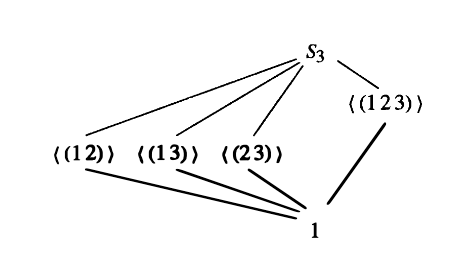
\includegraphics[width=.5\textwidth]{Sthree.png}
    \end{center}
  \end{figure} 
  \begin{proof}[Solution:] Clearly $C_{S_3}(1) = S_3$. Seeing how the centralizer of an element $x \in S_3$ is a subgroup 
    of $S_3$ containing $x$, by the way the lattice diagram is structured, $C_{S_3}((x))$ must be equal to either $\langle (x)\rangle$ or $S_3$.\\\\
    Consider $(12)$ and note that $(13)(12)(13) = (23)$, therefore $(13) \not\in C_{S_3}((12))$. Thus $C_{S_3}((12)) = \langle (12)\rangle$.\\\\
    Consider $(13)$ and note that $(12)(13)(12) = (23)$, therefore $(12) \not\in C_{S_3}((13))$. Thus $C_{S_3}((13)) = \langle (13)\rangle$.\\\\
    Consider $(23)$ and note that $(13)(23)(13) = (12)$, therefore $(13) \not\in C_{S_3}((23))$. Thus $C_{S_3}((23)) = \langle (23)\rangle$.\\\\
    Consider $(132)$ and note that $(13)(132)(13) = (123)$, therefore $(13) \not\in C_{S_3}((132))$. Since $(132) = (123)^2$, $C_{S_3}((132)) = C_{S_3}((123)) = \langle (123)\rangle$. 
  \end{proof}
\end{exercise}
\vspace{.15in}









\begin{exercise}[\textbf{2.5.8} - Stefano Fochesatto]
  \noindent
  \begin{enumerate}
    \item Find the normalizer of each subgroup in $S_3$.
    \begin{figure}[H] %\usepackage{float}
      \begin{center}
        \caption{Lattice Diagram for $S_{3}$}
        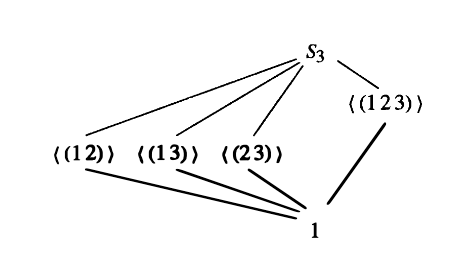
\includegraphics[width=.4\textwidth]{Sthree.png}
      \end{center}
    \end{figure} 
    \begin{proof}[Solution:]
      Clearly $N_{S_3}{\langle 1\rangle} = S_3$ and $N_{S_3}{\langle  S_3 \rangle} = S_3$. Similarly to the previous problem, since the normalizer of subgroup contains the subgroup,  and because of the structure of the lattice diagram for any subgroup $G$, 
      either $N_{S_3}(G) = G$ or $N_{S_3}(G) = S_3$.\\
    Consider $\langle 12\rangle$ and note that $(13)(12)(13) = (23)$. Since $(23) \not\in (\langle (12)\rangle)$ we know that $(13) \not\in N_{S_3}(\langle (12)\rangle)$ and therefore $N_{S_3}(\langle (12)\rangle) = \langle (12)\rangle$.\\\\
    Consider $\langle 13\rangle$ and note that $(12)(13)(12) = (23)$. Since $(23) \not\in (\langle (13)\rangle)$ we know that $(12) \not\in N_{S_3}(\langle (13)\rangle)$ and therefore $N_{S_3}(\langle (13)\rangle) = \langle (13)\rangle$.\\\\
    Consider $\langle 23\rangle$ and note that $(13)(23)(13) = (12)$. Since $(12) \not\in (\langle (23)\rangle)$ we know that $(13) \not\in N_{S_3}(\langle (23)\rangle)$ and therefore $N_{S_3}(\langle (23)\rangle) = \langle (23)\rangle$.\\\\
    Finally consider $\langle (123)\rangle = \{1, (123), (132)\}$, and note that
    \begin{equation*}
      (12)(123)(12) = (132),
    \end{equation*}
    \begin{equation*}
      (12)(132)(12) = (123).
    \end{equation*}
    Therefore, $(12) \in N_{S_3}(\langle (123)\rangle)$, and since $(12) \not\in \langle (123)\rangle$ we know that $N_{S_3}(\langle (123)\rangle) = S_3$. 
    \end{proof}
    \vspace{.15in}

    \item Find the normalizer of each subgroup in $Q_8$\\
   \begin{figure}[H] %\usepackage{float}
      \begin{center}
        \caption{Lattice Diagram for $Q_{8}$}
        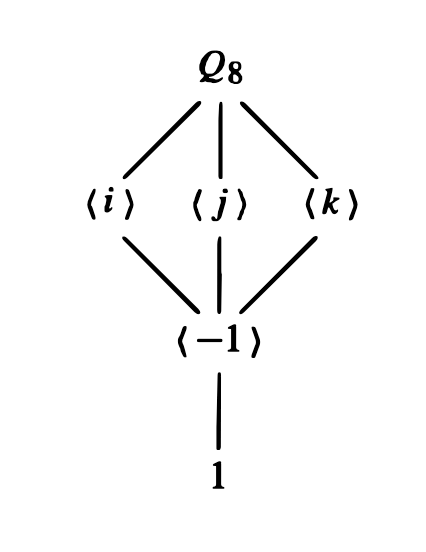
\includegraphics[width=.3\textwidth]{Qeight.png}
      \end{center}
    \end{figure} 
    \begin{proof}[Solution:] Clearly $N_{Q_8}(\langle 1\rangle) = Q_8$ and $N_{Q_8}(\langle  Q_8 \rangle) = Q_8$. Let $a\in Q_8$ and note that,
      $a(-1)a^{-1} = a(-1)(-1)a = a^2 = -1 \in \langle -1\rangle $. Thus  $N_{Q_8}(\langle -1\rangle) = Q_8$. Since the normalizer of subgroup contains the subgroup, and because of the structure of the lattice diagram for subgroups $G = \{\langle  i \rangle, \langle  j \rangle, \langle  k \rangle\}$, 
      either $N_{Q_8}(G) = G$ or $N_{Q_8}(G) = Q_8$.\\
      Consider $\langle  i \rangle$ and note that $ji(-j) = (-k)(-j) = -i \in \langle i\rangle $  and $j-i(-j) = (j)(k) = i \in \langle i\rangle $. Therefore $j \in N_{Q_8}(\langle  i \rangle)$, thus $N_{Q_8}(\langle  i \rangle) = Q_8$. \\\\
      Consider $\langle  j \rangle$ and note that $ij(-i) = (k)(-i) = -j \in \langle j\rangle $  and $i-j(-i) = (i)(-k) = j \in \langle j\rangle $. Therefore $j \in N_{Q_8}(\langle  j \rangle)$, thus $N_{Q_8}(\langle  j \rangle) = Q_8$. \\\\
      Consider $\langle  k \rangle$ and note that $ik(-i) = (-j)(-i) = -k \in \langle k\rangle $  and $i-k(-i) = (i)(j) = k \in \langle k\rangle $. Therefore $j \in N_{Q_8}(\langle  k \rangle)$, thus $N_{Q_8}(\langle  k \rangle) = Q_8$. 
    \end{proof}
  \end{enumerate}
\end{exercise}
\vspace{.15in}







\begin{exercise}[\textbf{3.1.24} - Stefano Fochesatto] Prove that if $N$ is a normal subgroup of $G$ and $H$ is any subgroup of $G$ then $N\cap H$
  is a normal subgroup of $H$.
  \begin{proof} Suppose $N$ is a normal subgroup of $G$ and $H$ is any subgroup of $G$. Let $a, b \in N\cap H$, clearly 
    $ab^{-1} \in  N\cap H$, hence $N\cap H \leq H$. Note that since $N$ is normal in $G$ and $H$ is a subgroup for all $h \in H$
    $hah^{-1} \in N$. Since $a \in H$ and $H$ is a subgroup we know that $hah^{-1} \in H$. Thus $hah^{-1} \in N\cap H$ and therefore 
    $N\cap H$ is normal in $H$. 
  \end{proof}
\end{exercise}
\vspace{.15in}








\begin{exercise}[\textbf{3.1.36} - Stefano Fochesatto] Prove that if $G/Z(G)$ is cyclic then $G$ is abelian. [If $G/Z(G)$ is cyclic 
  with generator $xZ(G)$, show that every element of $G$ can be written in the form $x^az$ for some integer $a \in \ZZ$ and some element $z \in Z(G)$.]
  \begin{proof} Suppose $G/Z(G) = \langle  xZ(G)\rangle$ for some fixed $x \in G$. Since $G/Z(G)$ is cyclic there exists some $a \in \ZZ$ such that for all $g \in G$, 
    \begin{equation*}
      gZ(G) = (xZ(G))^a = x^aZ(G). 
    \end{equation*}
    Now consider $a, b \in G$, and note since $Z(G)$ is a subgroup of $G$ we know $G/Z(G)$ forms a partition of $G$ and thus 
    $a$ and $b$ belong to some left coset of $Z(G)$. Therefore by the previous result there exists some 
    $\alpha, \beta \in \ZZ$ and $z_1, z_2 \in Z(G)$ such that $a = x^{\alpha}z_1$ and $b = x^{\beta}z_2$. Since $z_1, z_2$ are commute with every element in $G$, 
    \begin{equation*}
      ab = x^{\alpha}(z_1x^{\beta})z_2 = x^{\alpha + \beta}(z_1z_2) = x^{\alpha + \beta}z_2z_1 = x^{\beta}(x^{\alpha}z_2)z_1 = x^{\beta}z_2x^{\alpha}z_1 = ba
    \end{equation*}
  \end{proof}
\end{exercise}
\vspace{.15in}








  \end{document}